\section{ER-diagram}

ER-diagrammet vist i \autoref{fig:er-diagram} viser entiteter, relasjoner og attributter.

\begin{figure}[H]
    \centering
    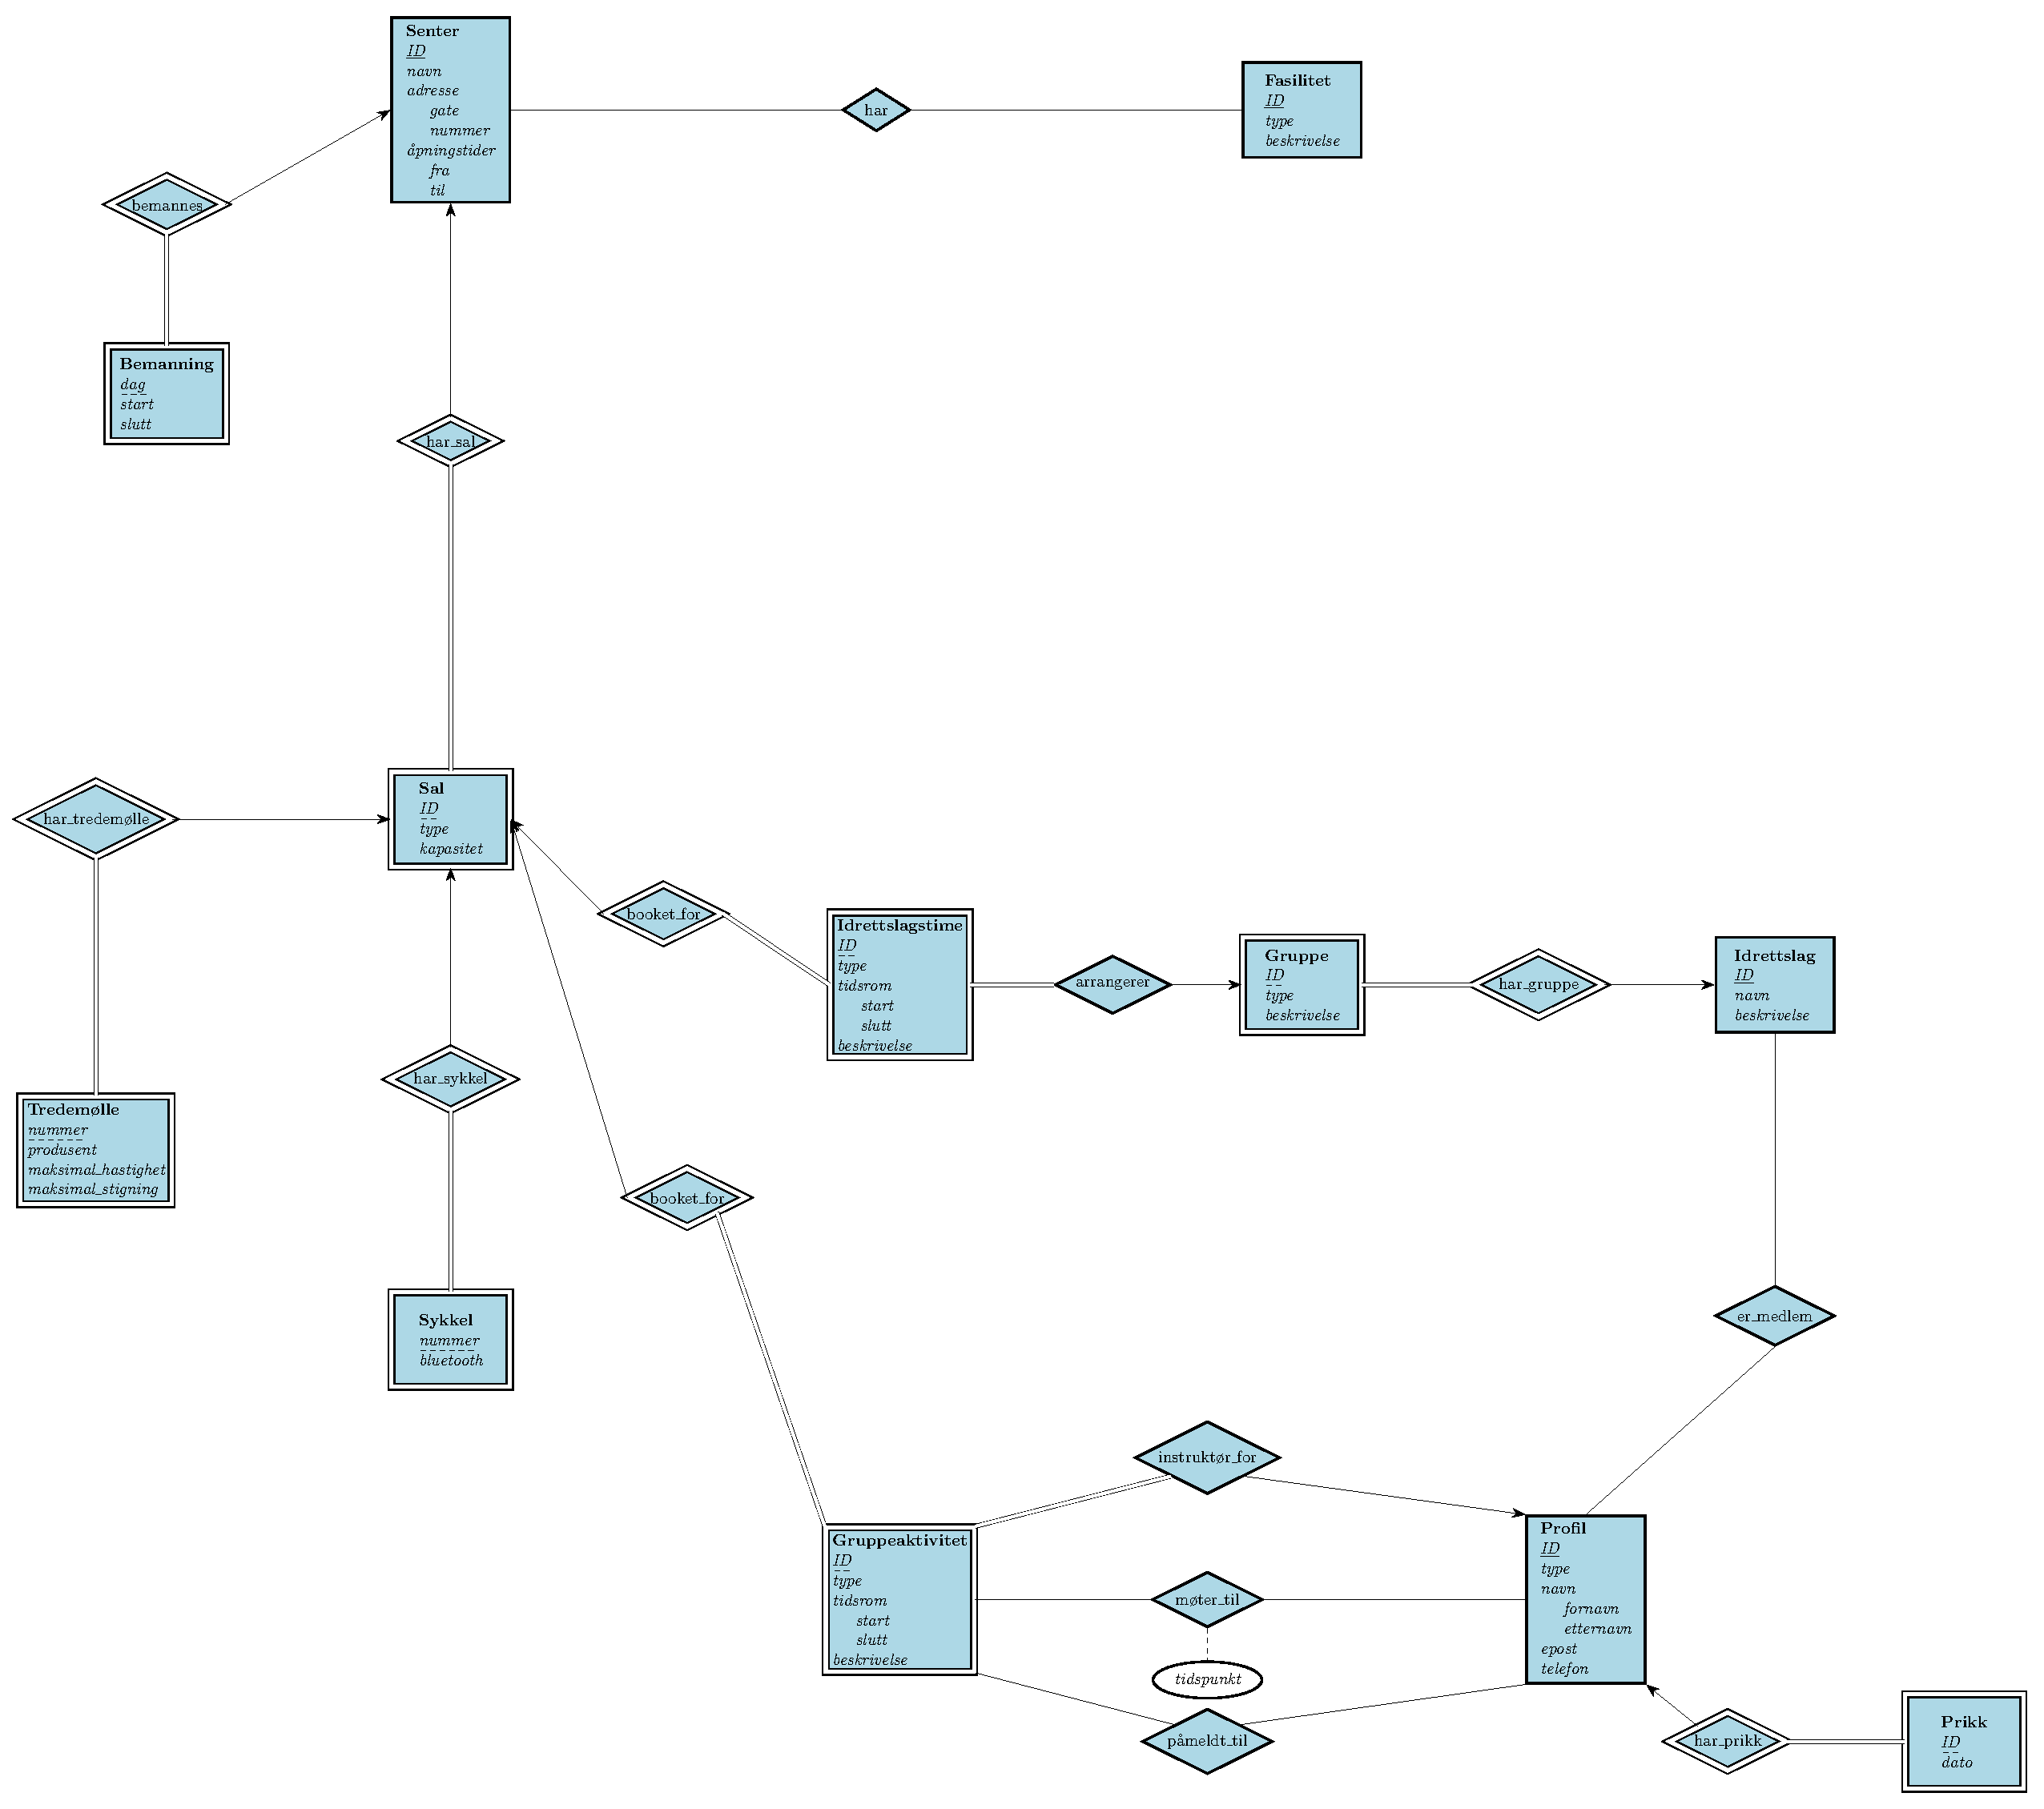
\includegraphics[width=\textwidth,height=0.95\textheight,keepaspectratio]{database-modeling/ER-diagram/ER-diagram.pdf}
    \caption{ER-diagram.}
    \label{fig:er-diagram}
\end{figure}

\subsection{Antakelser}

Følgende antakelser er gjort:

\begin{enumerate}
    \item \textbf{Fasiliteter.} Vi har én entitet for fasiliteter med \textit{type} som attributt (f.eks.\ badstue, garderobe, øvelsesrom). Problembeskrivelsen tolkes slik at det viktige er å beskrive hvilke fasiliteter senteret har, ikke attributtene til hver fasilitetstype. En alternativ modellering ville vært å splitte opp i flere entity sets.
    \item \textbf{Bemanning.} Bemanningstidspunktene antas like fra uke til uke; \textit{dag} er derfor brukt som diskriminator (eng, discriminator).
     Vi tolker at det viktige er \textit{når} senteret er bemannet,
      ikke hvem som bemanner. Bemanning kunne alternativt vært koblet til Profil.
      Et tredje alternativ ville vært å ha bemanning som en attributt for senteret.
      Ulempen med dette er at vi fort kunne fått null-verdier.
    \item \textbf{Plasser på aktivitet.} Antall plasser på en aktivitet er definert ut fra kapasiteten til salen aktiviteten foregår i.
    \item \textbf{Påmelding og kø.} Køsystemet i påmelding tilrettelegges for med et påmeldingsnummer, som fungerer som kølapp.
     For en aktivitet i en sal med kapasitet $n$ regnes de $n$ profilene med lavest påmeldingsnummer som påmeldt, resten står på venteliste.
     For idrettslagstime vil vi bruke et dropin-system, der de $n$ første som møter vil få plass.
    \item \textbf{Sykler og tredemøller.} Utstyr flyttes ikke mellom rom og identifiseres entydig med nummer og sal.
    \item \textbf{Instruktør.} Vi har generalisert Profil-entiteten, slik at dette fanger både ansatte/instruktører
     og vanlige medlemmer. Vi skiller mellom rollene med attributten \textit{type}. Dette kan forsvares med at instruktører
      potensielt også kan være medlemmer, og dermed delta på andre aktiviteter og være med i idrettslag. I praksis vil typen ansatt
       funke som et ekstra privilegie der profilen kan være instruktør for en aktivitet, men likevel har alle vanlige medlemsfunksjoner.
    \item \textbf{Idrettslagstime.} For en undergruppe av et idrettslag som arrangerer idrettslagstime, 
    antas det at en profil ikke trenger å være medlem av gruppen for å delta, altså at det holder at profilen er medlem av idrettslaget.
\end{enumerate}

\subsection{Det ER-modellen ikke uttrykker}

% --- Skriv her: Diskuter hva som ikke lar seg uttrykke i ER-modellen (f.eks. constraints, regler, tidsaspekter). ---
